\section{Theorie}
\label{sec:theorie}

Treffen Lichtquanten auf eine Metalloberfläche,
lösen sie, sofern ihre Energie ausreicht, Elektronen aus. \\

Um diesen, auch Photoeffekt genannten Effekt näher zu untersuchen,
kann der in \autoref{fig:abb1} dargestellte Aufbau verwendet werden.

\begin{figure}
    \centering
    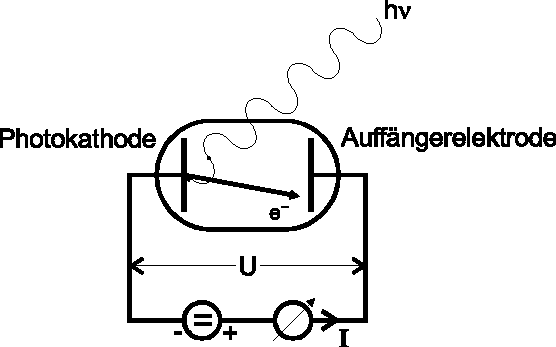
\includegraphics{figures/Abb1.pdf}
    \caption{Aufbau zur Untersuchung des Photoeffekts \cite{ap10}.}
    \label{fig:abb1}
\end{figure}

Bei Durchführungen dieses Versuches ergeben sich die folgenden Erkenntnisse:

\begin{enumerate}
    \item Die Zahl der pro Zeit ausgelösten Elektronen ist proportional zur Lichtintensität.
    \item Die Energie der Photoelektronen ist proportional zur Photonenfrequenz, aber unabhängig von der Lichtintensität.
    \item Unterhalb einer Grenzfrequenz tritt der Photoeffekt nicht auf.
\end{enumerate}
